\subsection{Grundlagen für die Realisierung}

Um sich die Freiheitsgrade der Realisierung von Verteilten Systemen bewusst zu werden, kann man sich im ersten Schritt noch einmal die grundsätzliche Architektur einer Recheneinheit vor Augen führen, die für die Problemlösung herangezogen werden kann. Typische Referenzen in diesem Fall sind die Harvard- oder die von-Neumann Architektur. 

Die Harvard-Architektur und die von-Neumann-Architektur sind beide grundlegende Architekturen für die Gestaltung von Computern und digitalen Rechensystemen. Beide Architekturen haben gemeinsam, dass sie die Grundlagen für die Funktionsweise moderner Computer bilden und auf der Verwendung von Binärcode und elektronischen Komponenten basieren.

Eine wichtige Unterscheidung besteht natürlich darin, dass die von Neumann-Architektur eine gemeinsame Speicherarchitektur hat, in der sowohl Anweisungen als auch Daten in einem gemeinsamen Speicher gespeichert werden. Die Harvard-Architektur hingegen verwendet getrennte Speicher für Anweisungen und Daten, was zu einem schnelleren Zugriff auf beide Arten von Informationen führen kann.
\\\\
Wie es auch sei,  beide Architekturen bieten einfach gesprochen ein Befehlssatz/Instruction Set Architecture (ISA), welches sich auf die spezifischen Anweisungen und Befehle bezieht, die ein Prozessor oder ein digitales Rechensystem ausführen kann, sowie die Möglichkeit der Datenrepräsentation, auf denen diese Anweisungen und Befehle basieren oder ausgeführt werden.
\\\\
Somit ergibt sich, das in einem Verteilten System\footnote{welches mindestens aus zwei Systemen besteht} die Notwendigkeit die Befehle oder Anweisung für eine kooperative Lösungsstrategie über ein Netzwerk zu addressieren. Die Herangehensweise an diese Herausforderung kann unterschiedlich interpritiert werden. Um die Strategien besser beurteilen zu können sollen zunächst die Zerlegungsmethoden und generellen Kommunikationsformen an den Schnittstellen diskutiert werden. 

\subsubsection{Funktionale vs. ressourcenorientierte Zerlegung}

In der Softwarearchitektur gibt es mehrere Teile-und-herrsche-Ansätze, um komplexe Systeme zu entwickeln und zu verwalten. Zunächst soll aber der Fokus auf eine Einteilung in zwei rudimentäre Ansätze gelegt werden:
\begin{itemize} 
\item Funktional
\item Ressourcenorientiert
\end{itemize}
Bei der funktionalen Zerlegung wird das System in kleinere, im besten Fall atomare, Funktionen/Prozeduren zerlegt, die jeweils auf eine bestimmte Aufgabe spezialisiert sind. Die Idee ist, dass jede Funkion unabhängig von den anderen funktioniert, um das System als Ganzes zu unterstützen. Beispielhaft könnte das eine Funktion sein, dass die Sortierung von Zahlen übernimmt, aber auch eine Funktion für die Filterung oder Suche. Die funktionale Zerlegung zielt darauf ab, die Komplexität des Systems zu reduzieren, indem es in kleinere, leichter handhabbare Teile aufgeteilt wird. 
Einfach gesprochen werden folgend disjunkte Funktionen bestimmt, versucht diese generisch zu erfassen und abstrahiert zu beschreiben. Eine Unterscheidung in \enquote{Funktionale}, \enquote{Deklarative} oder \enquote{Objektorientierte} Programmierung soll zu diesem Zweitpunkt noch nicht getroffen werden, da es auch in einem Verteilten System notwendig sein wird, unterschiedliche Programmierungsansätze miteinander zu verbinden. 
Zudem kann zu diesem Zeitpunkt auch mal festgestellt werden, dass die Auswahl der Sprache für die Lösung eines bestimmten Problems keine Rolle spielt, wenn alle beteiligten Sprachen Turing-vollständig sind. Das bedeutet, dass jede dieser Sprachen in der Lage ist, jede denkbare Berechnung durchzuführen, solange genügend Zeit und Speicherplatz zur Verfügung stehen.
\\\\
Richten wir weiter den Blick zunächst weiter auf Funnktionen und Prozesse. Für die Beschreibung von Funktionen/Prozessen gibt es eine recht generische Form, die über jeden Architekurtyp und jeder Sprache relativ konstant bleibt.
\begin{itemize} 
\item Funktionssignatur 
\item Funktionssemantik (Definition)
\end{itemize}
Ein Beispiel für die Formulierung einer Funktionssignatur in Pseudocode könnte für die Addition zweier Werte in dieser Form beschrieben werden:
\begin{lstlisting}[caption={Funktionssignatur},captionpos=b,label={lst:signatur}]
    function sum(a: int, b: int) -> int;
\end{lstlisting}
Die Funktionssignatur in Listing \ref{lst:signatur} gibt an, dass die Funktion \enquote{sum} zwei Parameter vom Typ \enquote{int} erwartet und einen Rückgabewert vom Typ \enquote{int} liefert. Einige der wichtigsten Informationen, die in einer Funktionssemantik enthalten sein können, sind:
\begin{itemize} 
\item Der Name der Funktion:\\ Dies gibt an, wie die Funktion genannt wird und welche Funktion sie ausführt.
\item Die Parameter der Funktion: Dies beschreibt, welche Eingabe die Funktion erwartet und welche Bedeutung die einzelnen Parameter haben.
\item Der Rückgabewert der Funktion:\\ Dies beschreibt, welche Ausgabe die Funktion liefert und welche Bedeutung der Rückgabewert hat.
\item Die Bedingungen und Einschränkungen:\\ Dies beschreibt, welche Bedingungen erfüllt sein müssen, damit die Funktion korrekt ausgeführt wird, und welche Einschränkungen es bei der Verwendung der Funktion gibt.
\item Die Ausführungslogik:\\ Dies beschreibt, wie die Funktion ausgeführt wird, welche Schritte dabei durchlaufen werden und welche Algorithmen verwendet werden.
\item Die Fehlerbehandlung:\\ Dies beschreibt, wie die Funktion mit Fehlern und Ausnahmen umgeht und welche Ausnahmen auftreten können.
\end{itemize} 
Die spezifischen Informationen, die in einer Funktionssemantik enthalten sind, hängen von der Art der Funktion und den Anforderungen der Anwendung ab, dennoch beschreibt auch die geringste Variante die Schnittstelle zu einem Teil des Befehlssatzes der zugrunde liegenden Architektur. 
\\\\
Die Funktionssemantik beschreibt die Bedeutung und den Zweck einer Funktion, nicht aber zwingend die Umsetzung auf dem Befehlssatz der Architektur. Sie beschreibt, was die Funktion tut und wie sie ausgeführt wird. Die Funktionssemantik kann in Form von Kommentaren, Dokumentation oder einfach durch den Code selbst ausgedrückt werden.
\begin{lstlisting}[caption={Funktionssemantik},captionpos=b,label={lst:semantik}]
    function sum(a: int, b: int) -> int {
        return a + b;
    }
\end{lstlisting}
Listing \ref{lst:semantik} beschreibt, dass die Funktion \enquote{sum} die beiden Parameter \enquote{a} und \enquote{b} addiert und das Ergebnis zurückgibt. In diesem Beispiel wird die Funktionssemantik durch den Code selbst ausgedrückt. Sind systematisch und vollständig alle atomaren Funktionen mit Funktionssignatur und Funktionssemantik in der Anforderungsanalyse und im Design bestimmt, kann aus der Summe aller Funktionen mit einer Funktionskomposition das gesamte System als die Summe aller Funktionen erstellt werden. Bei der Funktionskomposition werden Funktionen kombiniert, um komplexe Aufgaben zu erfüllen. Das Ergebnis der Funktionskomposition kann die erwartete Applikation sein, oder ein Teil des Gesamtdienstes (Service), der von dem Gesamtsystem erbracht werden soll. 
\\\\
Im Gegensatz dazu bezieht sich die ressourcenorientierte Zerlegung auf die Zerlegung des Systems in kleinere, auf Ressourcen orientierte Sicht. Die Idee ist, dass jede Einheit auf eine bestimmte Ressource spezialisiert ist und sie effizient nutzen kann, um das System als Ganzes zu unterstützen indem eine Schnittstelle zu der Ressource angeboten wird. Die Eigenschaften der Ressourcen werden typischerweise über ein reduziertes Set von Funktionen manipuliert.  In Bezug auf die ressourceorientierte Zerlegung ist CRUD\index{CRUD} ein wichtiger Teil des Entwurfsprozesses, da es die grundlegenden Operationen definiert, die auf Ressourcen angewendet werden können. Jede Ressource wird normalerweise mit einer oder mehreren der CRUD-Operationen verbunden sein.
Unter CRUD versteht man üblicherweise folgende Funktionen:

\begin{itemize}
\item \textbf{Create}: Erstellen oder Hinzufügen von neuen Daten in der Anwendung. Zum Beispiel kann ein Benutzer ein neues Konto erstellen oder ein Administrator kann einen neuen Datensatz hinzufügen.

\item \textbf{Read}: Lesen oder Abrufen von vorhandenen Daten aus der Anwendung. Zum Beispiel kann ein Benutzer seine Profilinformationen abrufen oder ein Mitarbeiter kann einen Bericht lesen.

\item \textbf{Update}: Aktualisieren oder Ändern von vorhandenen Daten in der Anwendung. Zum Beispiel kann ein Benutzer seine Profilinformationen aktualisieren oder ein Administrator kann die Kontaktinformationen eines Kunden ändern.

\item \textbf{Delete}: Löschen oder Entfernen von vorhandenen Daten aus der Anwendung. Zum Beispiel kann ein Benutzer sein Konto löschen oder ein Administrator kann einen ungenutzten Datensatz entfernen.
\end{itemize}
Die Schnittstelle einer Ressource muss nicht auf CRUD Funktionen reduziert sein, oder sie exakt in dieser Form umsetzen, aber wichtig ist dieses Konzept allemal.
\\\\

\begin{figure}[ht!]
  \centering
  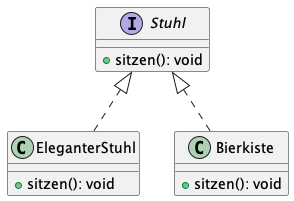
\includegraphics[width=0.4\textwidth]{fig/uml/stuhl-function.png}
  \caption{Funktionale Zerlegung mit Interface}
  \label{fig:stuhl-f}
\end{figure}

\begin{figure}[ht!]
  \centering
  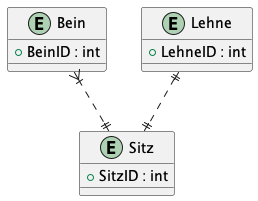
\includegraphics[width=0.4\textwidth]{fig/uml/stuhl-resourcen.png}
  \caption{Ressourcen-orientierte Zerlegung mit Relation}
  \label{fig:stuhl-r}
\end{figure}
Um den Unterschied der Ansätze nochmal zu verdeutlichen soll die Analogie der \enquote{Zerlegung eines Stuhls} als Sitzgelegenheit herangezogen werden. Wo bei der funktionalen Zerlegung die Suche nach einer Funktionen, wie das \enquote{Sitzen} im Vordergrund steht, und bei der ressourcenorientierten Zerlegung die Identifikation der einzlenen Ressourcen, wie (Stuhl-)Bein, Sitz(-fläche) oder (Rücken-)Lehne. Umgesetzt in ein Designentwurf für die funktionale Zerlegung ergibt sich beispielhaft in einer objektorientierten Sprache folgender der in dem Diagramm\ref{fig:stuhl-f} zu erkenne ist. 

In diesem Beispiel ist es wichtig zu erkennen, dass das Design mit der funktionalen Zerlegung auch seine Schwächen hat. Auch wenn eine korrekte Funktionssignatur bestimmt wurde, kann sich hinter dem Interface der realen Umsetzung dennoch eine nicht zu erwartende Umsetzung verbergen. In diesem  Beispiel wird beim Versuch sich zu setzen nicht nur ein eleganter Stuhl zu erwarten sein, sondern es kann auch eine Bierkiste die Sitzmöglichkeit repräsentieren. Diese Möglicheiten der Polymorphie eröffnet Chancen und Risiken.  
\\\\
Die ressourcenorientierte Zerlegung ist dahingehend intuitiver (siehe Abbildung \ref{fig:stuhl-r}, da ein System in seine einzelnen Ressourcen zerlegt wird, wobei diese eindeutig identifizierbar sein müssen. Auf diese Weise können diese Ressourcen als Entitäten Beziehungen zueinander aufbauen, welche wiederum mit weiteren Eigenschaften belegt werden können. In der korrekten Umsetzung ergibt sich so ein gutes Bild des Gesamtsystems. Die Gefahr besteht jedoch darin, dass die Ressourcen und deren Attribute nicht genau genug bestimmt werden oder die Beziehungen falsch beschrieben sind. In der hier benannten Analogie kann der Bausatz eines Stuhls auch auf eine Art und Weise beschrieben werden, dass die Lehne an den Beinen montiert ist und somit trotz identifizierter Ressourcen nicht den Dienst eines Stuhles, zumindest wie er erwartet wird, erfüllen kann.

Der geneigte Leser könnte als Übung hinterfragen, wie die Umsetzung eines Schachspiels in der funktionalen Zerlegung beschrieben werden könnte und wie dies in der ressourcenorientierten Zerlegung aussehen würde. So ergeben sich beispielhaft die Optionen, dass das Spielbrett sowohl in der objektorientierten Sprache durch eine Klasse mit Methoden ausgedrückt wird, die das Brett und die Spielregeln verwaltet, oder als Datenbankressource mit der gleichen Aufgabe.

Bei der Datenbank-Ressource werden die Spielzüge mit dem CRUD Interface realisiert. Spielregeln könnten durch Datenbank-Trigger erfasst werden. Ein Datenbank-Trigger ist ein spezielles Programm oder Skript, das  automatisch ausgeführt wird, wenn bestimmte Änderungen an einer Datenbanktabelle oder -sicht vorgenommen werden. Der Trigger wird auf eine bestimmte Aktion (z.B. INSERT, UPDATE oder DELETE) festgelegt und kann verwendet werden, um eine Reihe von Aufgaben oder Maßnahmen auszuführen, wenn diese Aktion auftritt.

\noindent\begin{minipage}{\textwidth}
\begin{lstlisting}[caption={Schachbrett - Objektorientiert},captionpos=b,label={lst:schachbrett-oo}]
public class ChessBoard {
    private Piece[][] board;

    public ChessBoard() {
        this.board = new Piece[8][8];
        // Initialize the board with the starting positions of pieces
        // e.g. add new Piece(PieceType.ROOK, Color.WHITE) to board[0][0] for the white rook in the top-left corner.
    }

    public Piece getPiece(int row, int col) {
        return board[row][col];
    }

    public void setPiece(int row, int col, Piece piece) {
        board[row][col] = piece;
    }

    // Other methods for checking if a move is valid, getting a list of possible moves, etc.
}
\end{lstlisting}
\end{minipage}

Die Wahl der richtigen Methode hängt von verschiedenen Faktoren ab, wie z.B. der Komplexität des Systems, der Art der Aufgaben, die ausgeführt werden müssen, und den verfügbaren Ressourcen.

Für die Zerlegung in einem verteilten System hat bereits die Auswahl der grundlegenden Strategie der Zerlegung einen hohen Einfluss. Die Schnittstellen der Systeme ändern sich dadurch und damit auch die notwendige Kommunikation und die Datenrepräsentation in den Systemen.\footnote{Eine weitere Art der Diskussion: \url{https://medium.com/double-pointer/system-design-interview-a-two-player-online-chess-game-4a150ad8ea78} }

\noindent\begin{minipage}{\textwidth}
\begin{lstlisting}[caption={Schachbrett - Datenbank},captionpos=b,label={lst:schachbrett-datenbank}]

CREATE TABLE ChessBoard (
    id INT PRIMARY KEY,
    row INT,
    col INT,
    pieceType VARCHAR(10),
    pieceColor VARCHAR(5)
);
\end{lstlisting}
\end{minipage}


\subsubsection{Datenseparation}

Die Datenseparation in verteilten Systemen bezieht sich auf den Prozess, bei dem Daten auf mehrere Knoten in einem Netzwerk verteilt werden, um die Leistung, Skalierbarkeit und Zuverlässigkeit des Systems zu verbessern. Dies wird typischerweise durch die Aufteilung von Daten in kleine Teile und deren Verteilung auf verschiedene Knoten oder Server im Netzwerk erreicht.
Es gibt verschiedene Möglichkeiten, Daten in verteilten Systemen zu separieren, einschließlich:
\begin{itemize}
\item \textbf{Horizontale Partitionierung}\index{Horizontale Partitionierung}: Hierbei wird eine Tabelle in mehrere kleinere Tabellen aufgeteilt und jede Teilung wird auf einem separaten Server gespeichert. Zum Beispiel könnte man Kundeninformationen basierend auf Regionen oder Alphabeten auf verschiedene Server verteilen.

Ein Beispiel für ein Unternehmen, das Horizontale Partitionierung einsetzt, ist Facebook. Facebook speichert seine Daten in einer horizontal partitionierten Datenbank, bei der jede Tabelle in mehrere Teilbereiche aufgeteilt wird, wobei jeder Teilbereich nur bestimmte Zeilen enthält. Dies ermöglicht es Facebook, die Last auf mehrere Datenbankserver zu verteilen und eine bessere Skalierbarkeit zu erreichen. Wenn ein Benutzer beispielsweise eine Suche durchführt, kann Facebook nur die benötigten Zeilen abfragen und somit eine schnellere Antwortzeit erzielen.
\item \textbf{Vertikale Partitionierung}\index{Vertikale Partitionierung}: Hierbei werden bestimmte Spalten einer Tabelle auf verschiedene Server verteilt. Zum Beispiel könnten personenbezogene Daten (Name, Geburtsdatum, Adresse usw.) auf einem Server gespeichert werden, während andere Daten wie Kontaktinformationen auf einem anderen Server gespeichert werden.

Ein Beispiel für eine Anwendung, die Vertikale Partitionierung einsetzt, ist die Online-Shop-Plattform Amazon. Amazon speichert seine Daten in einer vertikal partitionierten Datenbank, bei der jede Tabelle in mehrere Teilbereiche aufgeteilt wird, wobei jeder Teilbereich nur bestimmte Spalten enthält. Wenn ein Benutzer beispielsweise eine Suche nach einem bestimmten Produkt durchführt, kann Amazon nur die benötigten Spalten abfragen und somit eine schnellere Antwortzeit erzielen.

Ein weiteres Beispiel ist LinkedIn, die auch Vertikale Partitionierung nutzen, um ihre Datenbank effizienter zu gestalten. LinkedIn speichert ihre Nutzerdaten in verschiedenen Datenbanken, die jeweils auf bestimmte Anwendungen und Funktionen zugeschnitten sind. Dadurch können sie die Ladezeiten reduzieren und eine bessere Skalierbarkeit erreichen.
\item \textbf{Sharding}\index{Sharding}: Hierbei wird die Datenbank in kleine, unabhängige Teile aufgeteilt, die auf verschiedenen Servern gespeichert werden. Dies ermöglicht eine horizontale Skalierung und verbessert die Leistung des Systems. Sharding ist eine Art der horizontalen Partitionierung, die Daten auf der Grundlage eines Sharding-Schlüssels aufteilt.

Slack ist ein Beispiel für eine Anwendung, die eine Form des Sharding verwendet, um ihre Datenbankleistung zu skalieren. Sharding ist eine Technik, bei der eine Datenbank in mehrere Teilbereiche aufgeteilt wird, die als \enquote{Shards} bezeichnet werden. Jeder Shard enthält einen Teil der Daten, so dass die Datenbank effizienter und schneller durchsucht werden kann.

In Slack wird Sharding verwendet, um die Benutzerdaten zu partitionieren. Das bedeutet, dass die Daten der Benutzer in mehrere Shards aufgeteilt werden, um die Last auf mehrere Datenbankserver zu verteilen. Jeder Shard ist dabei in der Lage, seine eigene Last zu verarbeiten und kann unabhängig von den anderen Shards skaliert werden. Dadurch kann Slack eine höhere Skalierbarkeit und eine bessere Leistung erzielen.
\item Daten-\textbf{Replikation}: Hierbei werden Daten auf mehreren Knoten im Netzwerk gespeichert, um Redundanz und Fehlertoleranz zu gewährleisten. Wenn ein Knoten ausfällt, kann ein anderer Knoten die Arbeit übernehmen und sicherstellen, dass das System weiterhin funktioniert.
\end{itemize}
Die Datenseparation in verteilten Systemen ist ein wichtiger Aspekt für die Skalierung und die Verfügbarkeit von Anwendungen. Durch die Verteilung von Daten auf mehrere Knoten im Netzwerk kann das System schnell auf Anforderungen reagieren und bietet eine hohe Verfügbarkeit, selbst wenn einzelne Knoten ausfallen.

\subsubsection{Schnittstellen zwischen den Entitäten}

Verteilte Systeme bestehen aus mehreren eigenständigen \enquote{nodes}, die über ein Netzwerk miteinander verbunden sind und gemeinsam arbeiten. Jede node repräsentiert eine Funktion oder eine Ressource, bzw. die Orchestrierung im funktionalen bzw. ressource-orientierten Ansatz. Unabhängig der Zerlegungsmethode müssen diese nodes miteinander kommunizieren, um Daten auszutauschen und ihre Arbeit zu koordinieren. Hier sind einige Gründe, warum verteilte Systeme Kommunikation benötigen:

\begin{itemize}
\item Datenaustausch: In verteilten Systemen müssen Daten zwischen verschiedenen Computern ausgetauscht werden, um eine gemeinsame Aufgabe zu erfüllen. Beispielsweise müssen Datenbanken in verschiedenen Computern synchronisiert werden, damit jeder Computer auf die aktuellste Version der Daten zugreifen kann.
\item Ressourcenmanagement: In verteilten Systemen können Ressourcen wie Speicher, Prozessoren und Netzwerkbandbreite auf verschiedene Computer verteilt werden. Um diese Ressourcen effektiv zu nutzen, müssen die Computer miteinander kommunizieren und Ressourcenanforderungen und -freigaben koordinieren.
\item Koordination: In verteilten Systemen müssen die Computer miteinander kommunizieren, um Aufgaben zu koordinieren. Beispielsweise können sie Nachrichten austauschen, um sicherzustellen, dass jeder Computer über den Fortschritt der Aufgabe informiert ist und seinen Teil der Arbeit erledigt.
\item Fehlererkennung und -behebung: In verteilten Systemen kann ein Computer ausfallen oder fehlerhaft arbeiten. Die verbleibenden Computer müssen miteinander kommunizieren, um den Fehler zu erkennen und die Arbeit neu zu verteilen oder den fehlerhaften Computer auszuschließen.
\item Skalierung: In verteilten Systemen kann die Anzahl der Computer erhöht werden, um die Leistung zu verbessern oder um mit einer höheren Last umzugehen. Um diese Skalierbarkeit zu erreichen, müssen die Computer miteinander kommunizieren und ihre Arbeit effektiv aufteilen.
\end{itemize}    

\textbf{Kommunikation ist in verteilten Systemen unerlässlich}, somit muss diskutiert werden, welche Art der Kommunikation Unterstützung findet. Zunächst müssen aber die Freiheitsgrade identifiziert werden. 
Eine wesentliche Unterscheidung ist synchron und asynchron. Dies bezieht sich auf die Art und Weise, wie Informationen zwischen Systemen oder Komponenten über ihre Schnittstellen (Interfaces) ausgetauscht werden. Hier sind die Unterschiede zwischen synchrone und asynchrone Kommunikation:

\begin{itemize} 
\item Synchrone\index{synchrone} Kommunikation bedeutet, dass die Kommunikation in (beinah) Echtzeit stattfindet, d.h. der Sender wartet auf eine Antwort des Empfängers, bevor er mit der nächsten Aktion fortfährt. Beispielsweise kann eine Anwendung eine Anforderung an eine Datenbank senden und auf die Antwort der Datenbank warten, bevor sie mit der Verarbeitung der nächsten Anforderung fortfährt. Bei synchroner Kommunikation kann das System oder die Anwendung nur dann fortfahren, wenn die Antwort vollständig ist.
\item Asynchrone\index{asynchrone} Kommunikation hingegen bedeutet, dass die Kommunikation asynchron oder zeitversetzt erfolgt, d.h. der Sender sendet eine Nachricht an den Empfänger, ohne auf eine sofortige Antwort zu warten. Der Empfänger verarbeitet die Nachricht dann und sendet eine Antwort zurück, wenn er bereit ist. Beispielsweise kann eine Anwendung eine Anforderung an einen Server senden und ohne auf eine Antwort zu warten, mit der Verarbeitung der nächsten Anforderung fortfahren. Die Antwort des Servers wird später empfangen, wenn sie verfügbar ist.
\end{itemize}  
Synchrone Kommunikation ist einfach zu implementieren und zu kontrollieren, da der Sender auf eine Antwort des Empfängers wartet, bevor er fortfährt. Es ist jedoch langsam, da der Sender auf die Antwort des Empfängers warten muss, bevor er weitere Aktionen ausführen kann.

Asynchrone Kommunikation hingegen ist schneller, da der Sender die nächste Aktion ausführen kann, ohne auf die Antwort des Empfängers zu warten. Es ist jedoch schwieriger zu implementieren und zu kontrollieren, da der Sender und Empfänger möglicherweise nicht synchronisiert sind und es zu Datenverlust oder Fehlern kommen kann. \textbf{Bereits zu diesem Zeitpunkt sollte festgestellt werden, das ein Design mit asynchronen Aufrufen dennoch in Verteilten Systemen vorzuziehen ist}.
\\\\
Eine weitere Unterscheidung in der Kommunikation ist persistent\index{persistent} und transient\index{transient}. Persistente und transiente Kommunikation beziehen sich auf die Art und Weise, wie Daten in einem verteilten System übertragen werden und ob die Daten dauerhaft oder vorübergehend gespeichert werden.

Persistente Kommunikation bedeutet, dass die Daten, die zwischen den Systemen übertragen werden, dauerhaft gespeichert werden. Das bedeutet, dass die Daten im besten Fall auch nach einem Systemausfall oder einem Neustart des Systems noch verfügbar sind. Bei der persistenten Kommunikation wird die Datenübertragung oft über Protokolle wie das Transmission Control Protocol (TCP) abgewickelt, die sicherstellen, dass die Daten vollständig und fehlerfrei übertragen werden.

Transiente Kommunikation hingegen bedeutet, dass die Daten, die zwischen den Systemen uni- oder bidirektional übertragen werden, vorübergehend und nicht dauerhaft gespeichert werden. Das bedeutet, dass die Daten nach einem Systemausfall oder einem Neustart des Systems nicht mehr verfügbar sind. Transiente Kommunikation wird oft über Protokolle wie das User Datagram Protocol (UDP) abgewickelt, die schnell und effizient sind, aber keine Garantie dafür bieten, dass die Daten vollständig oder fehlerfrei übertragen werden.

Ein Beispiel für persistente Kommunikation ist die Übertragung von Daten zwischen einem Webserver und einer Datenbank. Die Daten, die von der Website an den Webserver gesendet werden, werden dauerhaft in der Datenbank gespeichert, damit sie jederzeit abgerufen werden können. Ein Beispiel für transiente Kommunikation ist das Streaming von Audio oder Video in Echtzeit, bei dem die Daten nur während des Streams verfügbar sind und nicht gespeichert werden müssen.
\\\\
Signal, Event und Nachricht sind drei Begriffe, die oft in der Informatik im Kontext der Kommunikation verwendet werden und leicht verwechselt werden können. Hier sind ihre Unterschiede:

\begin{itemize}  
\item (Call-)\textbf{Event}\index{Event}:
Ein Event ist ein Ereignis, das in einer Anwendung oder einem System auftritt und von einem Benutzer, einem anderen Prozess oder einer anderen Anwendung ausgelöst werden kann. Events können zum Beispiel ein Mausklick, ein Tastendruck, ein Datenbankupdate oder ein Systemalarm sein. Anwendungen können auf diese Ereignisse reagieren, indem sie bestimmte Aktionen ausführen.
\begin{figure}[!h]
  \centering
  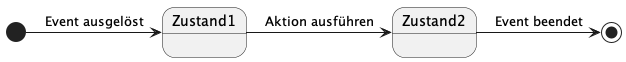
\includegraphics[width=0.95\textwidth]{fig/uml/simple-event.png}
  \caption{Einfaches Event}
  \label{fig:simple-event}
\end{figure}
Während ein Signal ein asynchrones Ereignis ist, ist ein (Call) Event im Allgemeinen synchron. Das bedeutet, dass wenn ein Objekt eine Operation auf einem anderen Objekt aufruft, die Kontrolle vom Sender an den Empfänger übergeben wird, bis die Operation abgeschlossen ist, woraufhin die Kontrolle zum Sender zurückkehrt. 

\item \textbf{Signal}\index{Signal}:
Ein Signal ist ein Ereignis, das von einem Betriebssystem oder einer Anwendung an eine andere Anwendung oder einen Prozess gesendet wird, um eine bestimmte Aktion auszulösen. Signale können zum Beispiel verwendet werden, um einen Prozess zu beenden, ein bestimmtes Verhalten auszulösen oder auf eine bestimmte Situation zu reagieren.
\begin{figure}[!h]
  \centering
  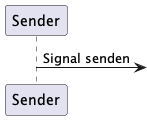
\includegraphics[width=0.25\textwidth]{fig/uml/simple-signal.png}
  \caption{Einfaches Signal}
  \label{fig:simple-signal}
\end{figure}
In der Modellierung der Architektur hat dies eine besondere Bedeutung, da ein Signal ein Objekt repräsentiert, das von einem Objekt asynchron ausgelöst wird und dann von einem anderen empfangen wird. Ein Beispiel hierfür sind Fehlerbehandlungen (Exceptions). Dem Signal ist keine Operation zugeordnet. Die Modellierung einer Klasse oder der Schnittstelle ist ein wichtiger Teil der Spezifikation. So kann definiert werden welches Signal durch die Operationen hinter einem Interface gesendet werden können.

\item \textbf{Nachricht}\index{Nachricht}:
Eine Nachricht ist eine Mitteilung, die von einer Anwendung, einem Prozess oder einem System an eine andere Anwendung, einen Prozess oder ein System gesendet wird. Nachrichten können zum Beispiel verwendet werden, um Daten zwischen verschiedenen Anwendungen oder Systemen auszutauschen, um einen bestimmten Prozess zu starten oder um Informationen über den Status eines Prozesses zu übermitteln. 
\begin{figure}[!h]
    \centering
    \begin{subfigure}[b]{0.45\textwidth}
      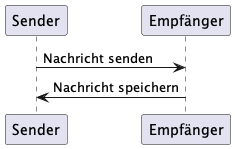
\includegraphics[width=0.8\textwidth]{fig/uml/async-message.png}
      \caption{Asynchrone Nachricht}
      \label{fig:async-msg}
    \end{subfigure}
    \hfill
    \begin{subfigure}[b]{0.45\textwidth}
        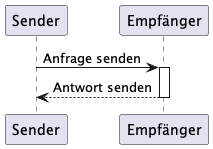
\includegraphics[width=0.75\textwidth]{fig/uml/sync-message.png}
        \caption{Synchrone Nachricht}
        \label{fig:sync-msg}
    \end{subfigure}
    \caption{}
    \label{fig:gesamt}
\end{figure}
\end{itemize}  
Bei Nachrichten gibt es normalerweise einen expliziten Sender und Empfänger, die durch Adressen oder IDs identifiziert werden. Der Sender sendet eine Nachricht an einen bestimmten Empfänger, der die Nachricht empfängt und darauf reagiert.

Dies soll auch nochmals mit den Events verglichen werden. Bei Events hingegen gibt es normalerweise keinen expliziten Sender oder Empfänger. Ein Event tritt auf, und Anwendungen oder Prozesse, die auf dieses Event hören, können darauf reagieren. 
\\\\
Weiter kann das versenden von Nachrichten sowohl synchron oder asynchron aufgefasst werden. Bei einem synchronen Aufruf exisitert eine Sende- und eine Empfangsnachricht. Bei einem asynchronen Aufruf, exisitert tyischerweise nur eine Sendenachricht.
\\\\
Signale und Events sind Ereignisse, die in einem System auftreten, während eine Nachricht eine Mitteilung ist, die zwischen verschiedenen Systemen ausgetauscht wird. Signale werden normalerweise zwischen verschiedenen Prozessen oder Anwendungen im selben System verwendet, während Events normalerweise innerhalb einer Anwendung auftreten. Nachrichten werden normalerweise zwischen verschiedenen Anwendungen oder Systemen ausgetauscht.

Events, Signale und Nachrichten bilden die Grundlage für weiterführende Konzepte in der Schnittstellenkonzeptionierung von verteilten Systmen:
\begin{itemize}  
\item \textbf{Remote Procedure Call} (RPC): Hierbei wird eine Funktion auf einem entfernten System aufgerufen, als ob sie lokal ausgeführt würde. Der Aufruf wird über das Netzwerk gesendet und das entfernte System führt die Funktion aus und gibt das Ergebnis zurück.
\item \textbf{Shared Memory}: Hierbei wird ein gemeinsamer Speicherbereich zwischen verschiedenen Knoten im System verwendet, auf den alle Knoten zugreifen können. Dadurch können Daten schnell und effizient zwischen Knoten geteilt werden.
\item \textbf{Datenbank-Replikation}: Hierbei werden Datenbanken auf verschiedenen Knoten im System repliziert, um die Verfügbarkeit und Skalierbarkeit zu verbessern. Änderungen an einer Datenbank werden automatisch an andere replizierte Datenbanken weitergeleitet, um sicherzustellen, dass alle Knoten im System auf dieselben Daten zugreifen können.
\item \textbf{Stream Processing}: Hierbei werden Daten in Echtzeit von verschiedenen Knoten im System gestreamt und verarbeitet, um Echtzeit-Analysen und -Verarbeitung zu ermöglichen. Stream Processing wird oft in Anwendungen wie Finanzdienstleistungen, E-Commerce und Social-Media-Anwendungen eingesetzt.
\end{itemize}  
Diese Möglichkeiten sollen auch mehr im Detail im Kontext der Architekturparadigmen diskutiert werden.

\subsubsection{Kopplung}
Bevor sich den Architekturen zugewendet wird, soll noch einige weitere wichtige Begriffe im Design verteilter Systeme eingebracht werden: Ein wichtiger ist der Kopplungsbegriff. 

Der Kopplungsbegriff ist in verteilten Systemen von entscheidender Bedeutung, da er die Art und Weise beschreibt, wie verschiedene Anwendungen und Systeme in einem verteilten System miteinander interagieren und kommunizieren. Eine falsche Wahl der Kopplungsart kann zu schwerwiegenden Problemen führen, die die Interoperabilität und Integration von Anwendungen in einem verteilten System beeinträchtigen können.
\\\\
Die Wahl der richtigen Kopplungsart kann jedoch auch erhebliche Vorteile bieten. Eine direkte Kopplung kann zu einer höheren Leistung führen und eine bessere Integration von Anwendungen ermöglichen, während eine indirekte Kopplung die Skalierbarkeit und Zuverlässigkeit verbessern kann. Eine losgekoppelte Architektur kann die Flexibilität  und die Ausfallsicherheit erhöhen, während eine strukturelle Kopplung die Zusammenarbeit und Integration von Anwendungen erleichtern kann. Im Detail ist es nochmal in der Tabelle\ref{tab:kopplungsarten} nochmal diskutiert.
\\\\
\begin{table}[!h]
  \centering
  \caption{Kopplungsarten in verteilten Systemen}
  \label{tab:kopplungsarten}
  \begin{tabular}{|p{4cm}|p{7cm}|}
    \hline
    \textbf{Kopplungsart} & \textbf{Beschreibung} \\ \hline
    Direkte Kopplung & Die Anwendungen und Systeme in einem verteilten System sind direkt miteinander verbunden und kommunizieren direkt miteinander. \\ \hline
    Indirekte Kopplung & Die Anwendungen und Systeme in einem verteilten System kommunizieren über ein gemeinsames Mediator-System oder eine Middleware miteinander. \\ \hline
    Losgekoppelte Kopplung & Die Anwendungen und Systeme in einem verteilten System kommunizieren über Nachrichten, ohne sich direkt zu verbinden. \\ \hline
    Strukturelle Kopplung & Die Anwendungen und Systeme in einem verteilten System sind durch gemeinsame Datenstrukturen oder Datentypen verbunden. \\ \hline
  \end{tabular}
\end{table}
Eine direkte Kopplung tritt auf, wenn Anwendungen oder Systeme direkt miteinander verbunden sind und direkt miteinander kommunizieren. Beispielsweise können zwei Anwendungen über eine Netzwerkverbindung oder einen direkten Datenlink verbunden sein und direkt miteinander kommunizieren.
\\
Eine indirekte Kopplung tritt auf, wenn Anwendungen oder Systeme über ein gemeinsames Mediator-System oder eine Middleware miteinander kommunizieren. Das Mediator-System oder die Middleware stellt eine Abstraktionsschicht bereit, die die Interoperabilität und Integration von Anwendungen in einem verteilten System erleichtert.

Eine losgekoppelte Kopplung tritt auf, wenn Anwendungen oder Systeme über Nachrichten kommunizieren, ohne sich direkt zu verbinden. In diesem Fall sendet eine Anwendung eine Nachricht an eine Middleware oder einen Broker, der die Nachricht an die Empfängeranwendung weiterleitet.

Eine strukturelle Kopplung tritt auf, wenn Anwendungen oder Systeme durch gemeinsame Datenstrukturen oder Datentypen verbunden sind. Beispielsweise können Anwendungen über eine gemeinsame Datenbank oder eine gemeinsame Dateistruktur kommunizieren. Die Tabelle~\ref{tab:kopplungsarten} gibt nochmals einen Überblick mit den Definitionen. 

\subsubsection{Mechanismen und Policies}

Mechanismen\index{Mechanismen} sind die grundlegenden Bausteine oder Funktionen, die zur Implementierung von verteilten Systemen benötigt werden. Policies hingegen sind die Entscheidungsregeln oder Leitlinien, die bestimmen, wie die Mechanismen eingesetzt und betrieben werden.
\\\\
Beispiele von Mechanismen in verteilten Systemen:
\begin{itemize} 
\item Kommunikation: In verteilten Systemen müssen die Knoten miteinander kommunizieren, um Daten auszutauschen und zusammenzuarbeiten. Mechanismen wie Message Passing, Remote Procedure Calls (RPC) und Remote Method Invocation (RMI) ermöglichen diese Kommunikation.
\item Synchronisation: Da verteilte Systeme aus mehreren unabhängigen Knoten bestehen, ist es wichtig, ihre Aktionen und Ressourcenzugriffe zu synchronisieren. Mechanismen wie Locks, Semaphore, Monitore und Barrieren werden verwendet, um die Synchronisation zu erreichen.
\item Replikation: Die Replikation ist ein Mechanismus, bei dem Daten oder Dienste auf mehreren Knoten im verteilten System dupliziert werden, um die Verfügbarkeit, Fehlertoleranz und Leistung zu verbessern.
\item Konsistenz: Um die Datenintegrität in verteilten Systemen aufrechtzuerhalten, müssen Mechanismen zur Gewährleistung der Konsistenz der Daten eingesetzt werden. Beispiele sind sequentielle Konsistenz, kausale Konsistenz, eventual Konsistenz und ACID-Transaktionen.
\end{itemize} 
Beispiele von Policies\index{Policies} in verteilten Systemen:
\begin{itemize} 
\item Ressourcenallokation: In verteilten Systemen müssen Entscheidungen darüber getroffen werden, wie Ressourcen wie Rechenleistung, Speicherplatz und Bandbreite zugewiesen werden. Beispiele für Ressourcenallokations-Policies sind First-Come-First-Served (FCFS), Round Robin, Prioritätswarteschlangen und Fair-Share-Scheduling.
\item Fehlerbehandlung: Policies zur Fehlerbehandlung legen fest, wie verteilte Systeme auf Fehler wie Hardware- oder Softwareausfälle, Netzwerkstörungen oder Datenverlust reagieren. Beispiele für Fehlerbehandlungspolicies sind Retry, Timeout, Fallback auf Alternativen und Datenwiederherstellung.
\item Sicherheit: Sicherheits-Policies bestimmen, wie verteilte Systeme den Schutz von Daten, Diensten und Benutzern gewährleisten. Beispiele sind Authentifizierung, Autorisierung, Verschlüsselung und Auditing.
\item Lastverteilung: Lastverteilungspolicies legen fest, wie die Arbeitslast in verteilten Systemen auf die verschiedenen Knoten verteilt wird, um eine optimale Leistung und Ressourcenauslastung zu erreichen. Beispiele sind statische Lastverteilung, dynamische Lastverteilung und adaptives Load Balancing.
\end{itemize}     

Als Beispiel für die Ausprägung soll die Lastverteilung in einem verteilten System gewählt sein, welche genutzt wird um einen  Webserver-Cluster zu betreiben. In diesem Fall ist Lastverteilung zunächst ein Mechanismus, der die Arbeitslast über mehrere Server oder Knoten verteilt, um eine bessere Leistung, Verfügbarkeit und Skalierbarkeit zu erreichen. Um eine effektive Lastverteilung zu ermöglichen, kann ein Load Balancer eingesetzt werden. Der Load Balancer ist dafür verantwortlich, ankommende Anfragen an die verschiedenen Server im Cluster weiterzuleiten.
Zudem kann die Policy darin bestehen, zu entscheiden, wie die Lastverteilung durchgeführt werden soll. Es gibt verschiedene Policies, die angewendet werden können, wie z. B. Round Robin, Least Connections oder Weighted Round Robin.
\begin{itemize} 
\item Round Robin: Der Load Balancer verteilt die Anfragen gleichmäßig auf alle verfügbaren Server, indem er sie der Reihe nach an jeden Server sendet.
\item Least Connections: Der Load Balancer leitet Anfragen an den Server weiter, der derzeit die wenigsten aktiven Verbindungen hat.
\item Weighted Round Robin: Der Load Balancer verteilt die Anfragen basierend auf dem Gewicht jedes Servers, das normalerweise die Kapazität oder Leistungsfähigkeit des Servers widerspiegelt.
\end{itemize}  
In diesem Beispiel ist der Lastverteilungsmechanismus (Load Balancer) für die Verteilung der Arbeitslast auf die verschiedenen Server im Cluster verantwortlich, während die Lastverteilungspolicy die Methode bestimmt, nach der die Verteilung erfolgen soll (Round Robin, Least Connections oder Weighted Round Robin). Die Policy kann je nach den spezifischen Anforderungen und Zielen des verteilten Systems ausgewählt und angepasst werden, diese Auswahl für jeden Mechanismus anzubieten, kann die Komplexität der Gesamtanwendung aber auch extrem steigern, so das mit einem Mechanismus nicht selten auch direkt die Policy im Mechanismus festgeschrieben wird.  

Ein anderes Beispiel ist näher an der Programmierung. Ein Vergleich zwischen einer API, die die Methoden left, right, up und down verwendet (Variante I), und einer API, die die Methode move(direction) verwendet (Variante II). Variante I ist in der Regel einfacher und direkt, da jede Methode jeweils eine einzelne Bewegungsrichtung repräsentiert. Dies führt zu einer besseren Typsicherheit, da es unwahrscheinlicher ist, dass ungültige Richtungen verwendet werden. Der Nachteil dieser API besteht darin, dass sie aus vier separaten Methoden besteht, was den Code länger und weniger flexibel machen kann. Außerdem ist diese API weniger skalierbar, da für die Hinzufügung neuer Richtungen jeweils neue Methoden erstellt werden müssten.

Auf der anderen Seite erlaubt die API mit der move(direction) Methode mehr Flexibilität, da die gewünschte Richtung als Parameter übergeben wird. Dies erleichtert die Steuerung der Bewegung in verschiedenen Szenarien. Die Skalierbarkeit ist ebenfalls höher, da beim Hinzufügen neuer Richtungen einfach neue Richtungsparameter eingebracht werden können, ohne dass neue Methoden erstellt werden müssen. Da nur eine Methode vorhanden ist, ist der Code kürzer und einfacher zu warten. Der Nachteil dieser API besteht darin, dass sie eine geringere Typsicherheit aufweist, da die Richtung als Parameter übergeben wird und somit die Möglichkeit besteht, dass ungültige oder unerwartete Richtungen verwendet werden.

\subsubsection{Stateful und stateless}
In verteilten Systemen beziehen sich die Begriffe \enquote{stateful}\index{stateful} und \enquote{stateless}\index{stateless} auf die Art und Weise, wie Systemkomponenten den Zustand ihrer Interaktionen verwalten.
\\\\
\textbf{Stateful}:\\
Ein stateful System speichert Informationen über den aktuellen Zustand der Kommunikation zwischen den Komponenten. Das bedeutet, dass ein stateful Service oder eine stateful Anwendung auf vorherige Anfragen oder Interaktionen Bezug nimmt und auf der Grundlage dieser Informationen reagiert. Stateful Systeme sind oft komplexer, da sie den Zustand der Interaktionen aktiv verwalten und speichern müssen. Sie können jedoch auch leistungsfähiger sein, da sie auf der Grundlage früherer Interaktionen individuellere oder optimierte Antworten liefern können.
\\\\
\textbf{Stateless}:\\
Ein stateless System speichert keine Informationen über den aktuellen Zustand der Kommunikation zwischen den Komponenten. Jede Anfrage oder Interaktion wird isoliert betrachtet, ohne Bezug auf frühere Anfragen oder Interaktionen. Stateless Systeme sind in der Regel einfacher zu implementieren und zu skalieren, da sie keine kontinuierliche Zustandsverwaltung erfordern. Sie können jedoch weniger leistungsfähig sein, wenn sie auf Informationen aus früheren Interaktionen angewiesen sind, um effektiv zu funktionieren.
\\\\
In verteilten Systemen können Nachrichtenabhängigkeiten einen Einfluss auf die stateful- oder stateless-Eigenschaften eines Systems haben. Nachrichtenabhängigkeiten treten auf, wenn die Verarbeitung einer Nachricht von der Verarbeitung einer oder mehrerer vorheriger Nachrichten abhängig ist. In solchen Fällen ist es erforderlich, den Zustand der Kommunikation zu verfolgen, um sicherzustellen, dass die Nachrichten in der richtigen Reihenfolge verarbeitet werden und das System korrekt funktioniert.
\begin{itemize}  
\item \textbf{Stateful Systeme}: Nachrichtenabhängigkeiten sind in stateful Systemen von Natur aus einfacher zu handhaben, da diese Systeme bereits den Zustand der Interaktionen verwalten. In stateful Systemen kann die Verarbeitung einer Nachricht auf früheren Nachrichten aufbauen, und das System kann sicherstellen, dass Nachrichten in der richtigen Reihenfolge verarbeitet werden.
\item \textbf{Stateless Systeme}: In stateless Systemen ist die Handhabung von Nachrichtenabhängigkeiten schwieriger, da kein Zustand zwischen den Anfragen gespeichert wird. Um Nachrichtenabhängigkeiten in stateless Systemen zu bewältigen, können Techniken wie das Hinzufügen von Sequenznummern oder Zeitstempeln zu Nachrichten verwendet werden, um die korrekte Reihenfolge der Nachrichtenverarbeitung sicherzustellen. In einigen Fällen müssen stateless Systeme den Zustand extern speichern oder verwalten, um Nachrichtenabhängigkeiten effektiv zu behandeln.
\end{itemize}  

Als ein Beispiel für einen zustandsbehafteten Dienst soll der Dateisystemserver eingebracht werden, welcher zuch Zustandsvariant ist.  Ein Dateisystemserver, der seinen Zustand oder seine Zustandsmaschine anpasst, basierend auf den empfangenen Nachrichten, kann daher als zustandsbehaftet oder stateful bezeichnet werden. In einem zustandsbehafteten System speichert der Server Informationen über die Interaktionen mit Clients, wie zum Beispiel offene Dateien, Positionen innerhalb von Dateien oder Benutzerberechtigungen.
\\\\
Wenn der Dateisystemserver eine Anfrage empfängt, z. B. zum Öffnen einer Datei, zum Lesen oder Schreiben von Daten oder zum Ändern von Berechtigungen, aktualisiert er seine Zustandsmaschine entsprechend. Die serverseitige Zustandsmaschine kann Informationen darüber enthalten, welche Dateien gerade geöffnet sind, welche Operationen auf ihnen ausgeführt werden und welche Benutzer Zugriff auf sie haben.

Durch das Beibehalten eines Zustands kann der Dateisystemserver effizienter arbeiten, da er die Informationen über die aktuellen Interaktionen und Operationen speichert und darauf zugreifen kann, ohne sie jedes Mal neu abrufen oder berechnen zu müssen. Allerdings bringt diese zustandsbehaftete Architektur auch Herausforderungen in Bezug auf Skalierbarkeit, Fehlertoleranz und Ressourcenverwaltung mit sich.

Die Wahl zwischen stateful und stateless Architekturen von den Anforderungen des verteilten Systems ab. Stateless Systeme bieten Vorteile in Bezug auf Einfachheit und Skalierbarkeit, während stateful Systeme besser für Anwendungen geeignet sind, bei denen der Kontext früherer Interaktionen für die korrekte Bearbeitung notwendig sind. 

\subsubsection{Transaktion}
In verteilten Systemen ist eine Transaktion eine Sequenz von Operationen, die auf verteilten Ressourcen oder Daten ausgeführt werden, um eine bestimmte Aufgabe oder Funktion zu erfüllen. Transaktionen sind wichtig, um die Konsistenz und Integrität von Daten in verteilten Systemen zu gewährleisten, insbesondere bei gleichzeitigen Zugriffen und Änderungen durch verschiedene Benutzer oder Prozesse.

Transaktionen in verteilten Systemen sollten die ACID-Eigenschaften (Atomicity, Consistency, Isolation, Durability) erfüllen:
\begin{itemize}
\item Atomicity (Atomarität): Eine Transaktion besteht aus einer Reihe von Operationen. Entweder werden alle Operationen erfolgreich ausgeführt und die Transaktion ist abgeschlossen, oder bei einem Fehler werden alle Operationen rückgängig gemacht, als ob die Transaktion nie stattgefunden hätte.
\item Consistency (Konsistenz): Transaktionen stellen sicher, dass das verteilte System von einem konsistenten Zustand in einen anderen konsistenten Zustand übergeht, auch wenn Fehler oder gleichzeitige Zugriffe auftreten.
\item Isolation (Isolierung): Jede Transaktion wird so ausgeführt, als ob sie isoliert von anderen gleichzeitig laufenden Transaktionen wäre. Dies bedeutet, dass die Zwischenergebnisse einer Transaktion für andere Transaktionen nicht sichtbar sind, bis die Transaktion abgeschlossen ist.
\item Durability (Dauerhaftigkeit): Sobald eine Transaktion abgeschlossen ist, sind ihre Änderungen dauerhaft im System gespeichert, selbst im Falle von Systemausfällen oder Fehlern.
\end{itemize}
Beispiele für Transaktionen in verteilten Systemen:
\begin{itemize}
\item Bankwesen: In einem verteilten Banksystem können Transaktionen verwendet werden, um Geldtransfers zwischen Konten durchzuführen. Die Transaktion stellt sicher, dass das Geld vom Senderkonto abgezogen und dem Empfängerkonto hinzugefügt wird, wobei die Konsistenz der Kontostände gewährleistet ist.
\item E-Commerce: In einem verteilten E-Commerce-System können Transaktionen verwendet werden, um Bestellungen und Zahlungen zu verarbeiten. Die Transaktion kann die Aktualisierung des Lagerbestands, die Berechnung von Steuern und Versandkosten, die Reservierung von Artikeln und die Verarbeitung der Zahlung beinhalten.
\item Verteilte Datenbanken: Bei verteilten Datenbanken werden Transaktionen verwendet, um sicherzustellen, dass mehrere Operationen, wie das Hinzufügen, Aktualisieren oder Löschen von Datensätzen, konsistent und gleichzeitig durchgeführt werden, ohne dass Inkonsistenzen oder Datenverluste auftreten.
\end{itemize}
Allerdings erfordert die Implementierung von Transaktionen in verteilten Systemen auch zusätzliche Überlegungen hinsichtlich Leistung, Fehlertoleranz und Koordination zwischen den beteiligten Knoten.
\\\\
Verschachtelte Transaktionen sind eine Erweiterung des grundlegenden Transaktionskonzepts, bei dem Transaktionen innerhalb einer übergeordneten Transaktion ausgeführt werden können. Diese innere Transaktion wird als \enquote{Untertransaktion} oder \enquote{Nested Transaction} bezeichnet. Eine verschachtelte Transaktion erlaubt es, dass Untertransaktionen unabhängig voneinander abgeschlossen oder abgebrochen werden, ohne die übergeordnete Transaktion als Ganzes zu beeinflussen.

Verschachtelte Transaktionen bieten Vorteile in Bezug auf Modularität, Fehlerbehandlung und Leistung, insbesondere in verteilten Systemen und bei komplexen Abläufen. Sie ermöglichen es, Teile einer größeren Transaktion separat abzuschließen und bei Fehlern nur die betroffenen Teile zurückzurollen, anstatt die gesamte Transaktion rückgängig zu machen.
\\\\
Ein Transaktionsmanager, auch als Transaktionskoordinator oder Transaktionsmonitor bezeichnet, ist eine Komponente in einem verteilten System, die für das Management und die Koordination von Transaktionen verantwortlich ist. Der Transaktionsmanager hat folgende Hauptaufgaben:
\begin{itemize}
\item Koordination: Der Transaktionsmanager koordiniert die beteiligten Ressourcen und Knoten in einer verteilten Transaktion, um sicherzustellen, dass sie konsistent und korrekt ausgeführt wird.
\item Protokollierung und Wiederherstellung: Der Transaktionsmanager führt ein Transaktionsprotokoll, um Änderungen und Aktivitäten während der Transaktion aufzuzeichnen. Im Falle eines Fehlers oder Systemausfalls verwendet der Transaktionsmanager das Protokoll, um den Zustand der beteiligten Ressourcen wiederherzustellen und die Transaktion entweder abzuschließen oder zurückzurollen.
\item Isolierung und Synchronisation: Der Transaktionsmanager stellt sicher, dass Transaktionen isoliert voneinander ausgeführt werden, um die Konsistenz und Integrität der Daten zu gewährleisten. Er ist auch für die Synchronisation von Zugriffen und Aktualisierungen auf verteilte Ressourcen verantwortlich, um Deadlocks und Konflikte zu vermeiden.
\item Commit und Rollback: Der Transaktionsmanager ist verantwortlich für das endgültige Commit (Abschluss) oder Rollback (Rückgängigmachung) einer Transaktion. Bei erfolgreicher Ausführung aller Operationen wird die Transaktion abgeschlossen und die Änderungen dauerhaft gespeichert. Im Falle eines Fehlers oder einer nicht erfüllten Bedingung führt der Transaktionsmanager einen Rollback durch, um die betroffenen Ressourcen in ihren vorherigen Zustand zurückzusetzen.
\end{itemize}
Ein Transaktionsmanager spielt eine entscheidende Rolle bei der Sicherstellung der Konsistenz, Integrität und Fehlertoleranz in verteilten Systemen, die Transaktionen verwenden. Das Konzept ist auch größer als aus einfachen Beispielen hervorgeht, die Bedeutung wird erst in der Flexibilität  deutlich. Dennoch soll ein Beispiel versucht werden, wo drei unabhängige Dienste: Flug, Hotel und Mietwagen zu einem neuen, vorher nicht vorhandenen Dienst zusammengefügt wird. 

Zuerst beginnt der Transaktionsmanager eine neue Transaktion. In dieser Transaktion werden die erforderlichen Ressourcen von den drei Diensten reserviert: Flugbuchung, Hotelbuchung und Mietwagenbuchung. Anschließend prüft der Transaktionsmanager, ob alle erforderlichen Ressourcen erfolgreich reserviert wurden und ob die Verfügbarkeit für den gewünschten Zeitraum gegeben ist.

Wenn alle Reservierungen erfolgreich sind und die Verfügbarkeit für den gewünschten Zeitraum bestätigt wurde, führt der Transaktionsmanager die Transaktion aus und erstellt die Urlaubsreise. Dabei wird der Gesamtpreis für Flug, Hotel und Mietwagen berechnet und dem Kunden in Rechnung gestellt. Nach erfolgreicher Zahlung bestätigt der Transaktionsmanager die Buchungen für die einzelnen Dienste und speichert die Informationen für die Urlaubsreise im System.

Falls jedoch eine oder mehrere Reservierungen nicht erfolgreich sind oder die Verfügbarkeit für den gewünschten Zeitraum nicht gegeben ist, wird der Transaktionsmanager die Transaktion abbrechen. In diesem Fall werden alle bisher reservierten Ressourcen für Flug, Hotel und Mietwagen freigegeben und der Kunde wird darüber informiert, dass die Urlaubsreise nicht erstellt werden konnte.

Der Transaktionsmanager stellt sicher, dass entweder alle Dienste erfolgreich kombiniert und die Urlaubsreise erstellt wird, oder keine der Reservierungen erfolgt und die Ressourcen wieder freigegeben werden. Dadurch wird ein konsistenter Zustand in den verteilten Systemen gewährleistet und es wird verhindert, dass teilweise reservierte oder unvollständige Urlaubsreisen entstehen.
\subsubsection{Message Passing}
Message Passing ist ein Kommunikationsparadigma in verteilten Systemen, bei dem Prozesse oder Komponenten Nachrichten austauschen, um Daten zu übertragen oder Aufgaben zu koordinieren. Es ist ein grundlegendes Konzept in der Kommunikation zwischen verteilten Einheiten und bildet die Basis für viele verteilte Systemarchitekturen, aber auch darüber hinaus.
Message Passing ist ein Konzept für die Nebenläufigkeits-Programmierung (Concurrent programming), der parallelen Programmierung (Parallel programming), der objektorientierten Programmierung und der Interprozesskommunikation.

Im Message Passing werden Nachrichten, die Daten oder Anweisungen enthalten, zwischen Prozessen oder Komponenten übermittelt. Die Kommunikation erfolgt in der Regel asynchron, d. h., der sendende Prozess wartet nicht darauf, dass der empfangende Prozess die Nachricht empfängt oder verarbeitet. Dies ermöglicht eine lose Kopplung der Komponenten und erleichtert die Skalierung und Fehlertoleranz des Systems. Die Eigenschaften von Message Passing können wie folgt zusammengefasst werden:
\begin{itemize}
\item Asynchrone Kommunikation: Die Kommunikation ist in der Regel asynchron, wodurch Prozesse unabhängig voneinander weiterarbeiten können, ohne auf Antworten warten zu müssen.
\item Lose Kopplung: Die Kommunikation zwischen Prozessen ist indirekt und erfordert keine direkte Kenntnis der beteiligten Prozesse, was zu einer losen Kopplung der Komponenten führt.
\item Skalierbarkeit: Message Passing eignet sich gut für verteilte Systeme mit einer großen Anzahl von Prozessen oder Komponenten, da es einfacher ist, zusätzliche Knoten hinzuzufügen und die Kommunikation zwischen ihnen zu verwalten.
\end{itemize}
Beispiele für Message Passing in verteilten Systemen:
\begin{itemize}
\item Message Queues: Message Queues sind Datenstrukturen, die zum Speichern und Übertragen von Nachrichten zwischen verteilten Prozessen verwendet werden. Beispiele für Message Queue-Systeme sind RabbitMQ, Apache Kafka und Amazon SQS. Sie ermöglichen die asynchrone Kommunikation und die Entkopplung von sendenden und empfangenden Prozessen.

\item Message Passing Interface (MPI): MPI ist ein Standard für die Kommunikation zwischen Prozessen in verteilten Systemen, insbesondere in High-Performance-Computing-Umgebungen. MPI stellt Funktionen zum Senden und Empfangen von Nachrichten, Synchronisation von Prozessen und Gruppenkommunikation bereit.

\item Publish-Subscribe-Systeme: In diesem Modell senden Publisher Nachrichten an Topics, während Subscriber Nachrichten von den Topics empfangen, die sie abonniert haben. Beispiele für Publish-Subscribe-Systeme sind Google Cloud Pub/Sub, Apache Pulsar und MQTT. Dieses Modell ist ereignisgetrieben und ermöglicht eine lose Kopplung der beteiligten Prozesse.
\end{itemize}
Message Passing ist ein grundlegendes Konzept in verteilten Systemen und ermöglicht die Kommunikation und Koordination zwischen Prozessen oder Komponenten in einer skalierbaren und fehlertoleranten Weise.

Das Actor-Modell ist ein Konzept für das Design von verteilten Systemen, das auf der Idee von unabhängigen Entitäten basiert, die als \enquote{Actoren} bezeichnet werden. Actoren sind grundlegende Recheneinheiten, die einen Zustand besitzen und in der Lage sind, Nachrichten zu empfangen und zu verarbeiten. Es setzt auf das Konzept von Message Passing auf. In diesem Modell kommunizieren Actoren ausschließlich über asynchrone Nachrichtenübermittlung, wodurch sie lose gekoppelt und hochgradig parallelisierbar sind. Die Hauptprinzipien des Actor-Modells sind:
\begin{itemize}
\item Isolation: Jeder Actor verwaltet seinen eigenen Zustand und verarbeitet Nachrichten unabhängig von anderen Actoren. Diese Isolation ermöglicht eine hohe Fehlertoleranz und erleichtert die Wartung und Skalierung des Systems.

\item Nachrichtenbasierte Kommunikation: Actoren kommunizieren über asynchrone Nachrichten. Nachrichten werden in Mailboxen abgelegt und von Actoren verarbeitet, wenn sie dazu bereit sind. Dieser Ansatz reduziert die Notwendigkeit von Locking- und Synchronisierungsmechanismen und ermöglicht eine hohe Parallelität.

\item Lokalitätstransparenz: Actoren können unabhängig von ihrer physischen Lage im verteilten System agieren. Die Kommunikation zwischen Actoren ist transparent und unabhängig von der Verteilung der Actoren im System.

\item Fehlertoleranz: Durch die Isolation der Actoren und ihre unabhängige Verarbeitung von Nachrichten können Fehler auf einzelne Actoren beschränkt bleiben, ohne das gesamte System zu beeinträchtigen. Das Actor-Modell unterstützt auch Supervision, bei der ein Actor die Verantwortung für das Überwachen und Wiederherstellen anderer Actoren bei Fehlern übernimmt.
\end{itemize}


\subsubsection{Idempotent}

Idempotenz\index{idempotenz} ist ein wichtiger Begriff in der Informatik und bezieht sich auf die Eigenschaft von Operationen, die wiederholt ausgeführt werden können, ohne dass sich das Ergebnis nach der ersten Anwendung ändert. Eine idempotente Operation ist eine, bei der das mehrmalige Anwenden auf dasselbe Eingabematerial das gleiche Ergebnis liefert, als ob sie nur einmal ausgeführt worden wäre.

Die Bedeutung von Idempotenz für verteilte Systeme liegt in ihrer Fähigkeit, die Robustheit und Zuverlässigkeit zu verbessern, insbesondere in Situationen, in denen Netzwerkfehler, Duplizierung von Nachrichten oder unvorhersehbare Verzögerungen auftreten können. In verteilten Systemen kann es schwierig sein, den genauen Zustand des Systems zu bestimmen, und es kann nicht garantiert werden, dass Nachrichten oder Anforderungen immer in der richtigen Reihenfolge oder genau einmal ankommen.

Indem idempotente Operationen in verteilten Systemen verwendet werden, können einige der Herausforderungen im Zusammenhang mit Fehlern und Unvorhersehbarkeiten bewältigt werden:
\begin{itemize}
\item Wiederholung von Anfragen: Wenn ein Client in einem verteilten System keine Antwort von einem Server erhält, kann es schwierig sein, festzustellen, ob die Anfrage verloren gegangen ist oder ob der Server die Anfrage einfach noch nicht verarbeitet hat. In solchen Fällen kann die Wiederholung einer idempotenten Anfrage ohne negative Auswirkungen erfolgen, da mehrmaliges Senden derselben Anfrage dasselbe Ergebnis wie das einmalige Senden liefert.
\item Fehlertoleranz: Idempotente Operationen können dazu beitragen, die Fehlertoleranz von verteilten Systemen zu erhöhen, indem sie die Auswirkungen von Nachrichtenduplikationen oder Netzwerkfehlern minimieren. Da idempotente Operationen dieselben Ergebnisse liefern, unabhängig davon, wie oft sie angewendet werden, können sie dazu beitragen, den Systemzustand trotz solcher Fehler konsistent zu halten.
\item Vereinfachung der Systementwicklung: Idempotenz kann dazu beitragen, die Komplexität von verteilten Systemen zu verringern, indem sie die Notwendigkeit von komplizierten Mechanismen zur Handhabung von Zustandsänderungen oder Fehlerbehebungen verringert. Da idempotente Operationen immer dieselben Ergebnisse liefern, unabhängig von ihrer Anwendungsreihenfolge, können Entwickler weniger Zeit damit verbringen, solche Mechanismen zu entwickeln, und sich stattdessen auf die Implementierung der Kernfunktionalität des Systems konzentrieren.
\end{itemize}

Ein Beispiel für die Verwendung von Idempotenz in verteilten Systemen ist das PUT-HTTP-Verb in HTTP-APIs. Das PUT-Verb wird verwendet, um eine Ressource mit einer bestimmten ID zu aktualisieren oder zu ersetzen. Wenn eine PUT-Anfrage mehrmals gesendet wird, bleibt das Ergebnis gleich, als ob die Anfrage nur einmal gesendet wurde. 


\subsubsection{Distributed Hash Table, DHT}

Distributed Hash Tables (DHTs\index{DHT}) sind ein Schlüssel-Wert-Speichersystem, das in verteilten Systemen eingesetzt wird. Sie bieten eine effiziente und dezentrale Möglichkeit, Schlüssel-Wert-Paare in einem Peer-to-Peer-Netzwerk zu speichern und abzurufen. In DHTs sind die Knoten des Netzwerks gleichberechtigt und es gibt keine zentrale Instanz, die die Speicherung und den Zugriff auf die Daten kontrolliert.

Die mathematische Grundlage von DHTs ist der konsistente Hashing-Algorithmus, der wie folgt dargestellt werden kann:

\begin{itemize}
\item Gegeben sei ein Schlüsselraum von $0$ bis $2^m - 1$, wobei $m$ die Anzahl der Bits ist, die zur Darstellung der Schlüssel verwendet werden.
\item Jeder Knoten und jeder Schlüssel im DHT wird durch eine eindeutige ID im Schlüsselraum repräsentiert. Die IDs können durch Hash-Funktionen wie z.B. SHA-1 erzeugt werden.
\item Die Knoten sind in einem logischen Ring angeordnet, basierend auf ihren IDs, der als "Ringraum" bezeichnet wird. Die Position eines Knotens im Ringraum wird durch seine ID bestimmt.
\item Um einen Wert für einen bestimmten Schlüssel zu speichern oder abzurufen, wird der Schlüssel zunächst durch dieselbe Hash-Funktion gehasht, die für die Erzeugung der Knoten-IDs verwendet wurde.
\item Der gehashte Schlüssel wird dann im Ringraum lokalisiert, und der zuständige Knoten für diesen Schlüssel ist derjenige, dessen ID gleich oder unmittelbar nach der gehashten Schlüssel-ID liegt. Dieser Knoten wird als \enquote{Verantwortlicher} für den Schlüssel bezeichnet.
\item Jeder Knoten speichert Informationen über eine kleine Anzahl anderer Knoten im Netzwerk, die als \enquote{Nachbarn} bezeichnet werden. Diese Nachbarn dienen zur Weiterleitung von Anfragen für Schlüssel, für die der aktuelle Knoten nicht verantwortlich ist.
\item Bei Änderungen im Netzwerk, wie zum Beispiel beim Hinzufügen oder Entfernen von Knoten, werden die Schlüssel-Wert-Paare entsprechend neu verteilt, um die Belastung gleichmäßig auf alle Knoten im Netzwerk zu verteilen.
\end{itemize}
